\documentclass[conference]{IEEEtran}
\IEEEoverridecommandlockouts
% The preceding line is only needed to identify funding in the first footnote. If that is unneeded, please comment it out.
\usepackage{cite}
\usepackage{amsmath,amssymb,amsfonts}
\usepackage{algorithmic}
\usepackage{graphicx}
\usepackage{textcomp}



\usepackage{multicol}% http://ctan.org/pkg/multicols
\usepackage{graphicx}% http://ctan.org/pkg/graphicx
\usepackage{float}
\usepackage{booktabs}
\usepackage{colortbl}
\usepackage{rotating}
\usepackage{multirow}
\usepackage{bigstrut}
\usepackage{fourier, erewhon}
\usepackage{geometry}
\usepackage{hyperref}
\usepackage{cite}
\usepackage [ table ]{ xcolor }


\def\BibTeX{{\rm B\kern-.05em{\sc i\kern-.025em b}\kern-.08em
    T\kern-.1667em\lower.7ex\hbox{E}\kern-.125emX}}
\begin{document}

\title{Art Enhancement/Restoration*\\
{\footnotesize \textsuperscript{*}SGN-12007 Introduction to Image and Video Processing
Project work}}


\author{\IEEEauthorblockN{Zeinab rezaei Yousefi \\ 256252}
\IEEEauthorblockA{\textit{Faculty of Biomedical Sciences and Engineering } \\
\textit{Tampere University of Technology}\\
Tampere, Finland \\
rezaeiyo@student.tut.fi}
}

\maketitle

\begin{abstract}
Image enhancement techniques have been widely used in many applications of image processing. The aim of image enhancement is to improve of the quality of images for human interpretation or to provide betetr input for other automated image processing techniques. 

In this project first I will introduce a few methods of image enhancement including histogram and intensity equalization, non-linear transformation functions such as median filter, color map and color balancing. Then I apply these methods on 10 chosen images and will discuss the results. 

\end{abstract}

\begin{IEEEkeywords}
image enhancement, image quality, contrast strechting, non-linear transformation, color balance\end{IEEEkeywords}

\section{Introduction}

The electronic, networked and interactive nature of the digital world has a significant impact on the arts.  The digital transition allows artists to replace physical objects with electronic files and to displace distribution over time and between places with instantaneous distribution over networks \cite{poole}. However, transferring the large-scale painting or sculpture into a digital file can lead to a degradation of their visual appearance and we all know that art should be studied and admired in the form the artist has made it. Thanks to developement of image processing, we can now benefit from different processing methods to enhance or restore the digitized artworks.    

The principal objective of image enhancement is to process a given image so that the result is more suitable than the original image for a specific application. It accentuates or sharpens image features such as edges, boundaries, or contrast to make a graphic display more helpful for display and analysis. The enhancement doesn't increase the inherent information content of the data, but it increases the dynamic range of the chosen features so that they can be detected easily\cite{gonzalez}.

When image enhancement techniques are used as pre-processing tools for other image processing techniques, then quantitative measures can determine which techniques are most appropriate. However, the greatest difficulty in image enhancement is quantifying the criterion for enhancement is empirical and requires interactive procedures to obtain satisfactory results.
Unfortunately, there is no general theory for determining what is ``good'' image enhancement when it comes to human perception.

The aim of this project is to apply different image enhancement methods on 10 different art images from the Web
Gallery of Art (\url{https://www.wga.hu/index1.html}) and devise a strategy to enhance and or restore (in grey
and or color) the selected art. Note that artificial noise or blurring is not being introduced in any of the images.  




% For each selected image (you are free to select any images to fulfil your needs), explain the reason why it was selected, what is your goal, what is your processing strategy and why,
%produce the output image(s) (can be more than one output) and measure your performance. 

There are different types of enhancement methods that can be applide to the images, such as:
\begin{itemize}
\item \textbf{Enhancement by point processing:} such as simple intensity transformation and histogram processing
\item \textbf{Spatial filtering:} such as smoothing filters and sharpening filters
\item \textbf{Enhancement in the frequency domain}
\item \textbf{Pseudo-color image processing}
\end{itemize}


%
%The operation can be formulated as
%g(x,y) =
%T[f(x,y)], where
%g is the output,
%f is the input image
%and
%T is an operation on
%f defined over some
%neighborhood of (x,y).
% According to the operations on the image pixels, it
%can be further divided into 2 categories: Point
%operations and spatial operations (including linear
%and non-linear operations).


\section{Methods and materials}
In this project I did not apply any frequency domain enhancement. In the following I explain the applied techniques briefly. 
\subsection{Intensity equalization}
Contrast is an important factor in any subjective evaluation of image quality. Contrast is created by the difference in luminance reflected from two adjacent surfaces. In other words, contrast is the difference in visual properties that makes an object distinguishable from other objects and the background. In visual perception, contrast is determined by the difference in the colour and brightness of the object with other objects. Many algorithms for accomplishing contrast enhancement have been developed and applied to problems in image processing.

Low-contrast images can result from poor illumination, lack of dynamic range in the image sensor, or even wrong setting of a lens aperture during image acquisition. The idea behind contrast stretching is to increase the dynamic range of the gray levels in the image being processed.

\subsection{Histogram equalization}

The histogram of a digital image with gray levels in the range $[0,L-1]$ is a discrete function $p(r_{k})=n_{k}/n$, where $r_{k}$ is the kth gray level, $n_{k}$ is the number of pixels in the image with that gray level, n is the total number of pixels in the image, and $k=0,1...,L-1$. $P(r_{k})$ gives an estimate of the probability of occurrence of gray level $r_{k}$.
The shape of the histogram of an image gives us useful information about the possibility for contrast enhancement. A histogram of a narrow shape indicates little dynamic range and thus corresponds to an image having low contrast \cite{gonzalez}.

Histogram equalization is a common technique for enhancing the appearance of images. Suppose we have an image which is predominantly dark. Then its histogram would be skewed towards the lower end of the grey scale and all the image detail is compressed into the dark end of the histogram. If we could stretch out the grey levels at the dark end to produce a more uniformly distributed histogram then the image would become much clearer. The objective is to map an input image to an output image such that its histogram is uniform after the mapping.
Histogram equalization only generates a approximation to a uniform histogram.

%Histogram equalization involves finding a grey scale transformation function that creates an output image with a uniform histogram (or nearly so).

\subsection{Spatial filtering}
The Spatial domain techniques are performed to the image plane itself and they are based on direct manipulation of pixels in an image.
The use of spatial masks for image processing is called spatial filtering. The masks used are called spatial filters. The basic approach is to sum products between the mask coefficients and the intensities of the pixels under the mask at a specific location in the image(2D convolution).

\subsubsection{Smoothing filter}

Smoothing filters are used for blurring and for noise reduction. Blurring is used in preprocessing steps, such as removal of small details from an image prior to object extraction, and bridging of small gaps in lines or curves. Noise reduction can be accomplishing by blurring with a linear filter and also by nonlinear filtering.

\subsubsection{Median filter}
If the objective is to achieve noise reduction instead of blurring, this method should be used.
This method is particularly effective when the noise pattern consists of strong, spike-like components and the characteristic to be preserved is edge sharpness.  

 For each input pixel $f(x,y)$, we sort the values of the pixel and its neighbors to determine their median and assign its value to output pixel $g(x,y)$. The outcome of median filtering is that pixels with outlying values are forced to become more like their neighbours, but at the same time edges are preserved. Median filtering is a nonlinear operation often used in image processing to reduce "salt and pepper" noise.


\subsection{Color balancing}

In image processing, color balance algorithm attempt to adjust the intensities of the colors (typically red, green, and blue primary colors). An important goal of this adjustment is to render specific colors  --particularly neutral colors-- correctly. Hence, the general method is sometimes called gray balance, neutral balance, or white balance. Color balance changes the overall mixture of colors in an image and is used for color correction \cite{wikiColorBalance}. 

\subsection{Pseudo coloring }
In automated image analysis, color is a powerful descriptor that often simplifies object identification and extraction from a scene. Human eye performs much better in discerning shades of color than gray scale. Therefore, transformation of a gray scale image into pseudo color image helps in better visualization of the image.

The main idea behind pseudo color transformation is to perform three independent transformation (RED,GREEN and BLUE) on the grayscale or intensity image and map  the corresponding intensity value in the image to the result obtained \cite{angel}.

In order to apply pseudo coloring, 3 independent transformations on the gray level of any input pixel need to be performed. Then the three results are fed separately into the R, G, B channels of a color monitor. 
This method produces a composite image whose color content is modulated by the nature of the transformation functions.


\section{Results and discussion}
In this section, 10 chosen original pictures from the Web Gallery of Art (\url{https://www.wga.hu/index1.html}) and the results of applying the above methods on these pictures are shown. 
In the two first figures (Fig.\ref{int_1} and Fig.\ref{int_2}), first I convert the RGB image into HSV and then equalization is applied to the luminance or value channel without resulting in changes to the hue and saturation of the image. As it can be seen in both figures the darkness of the original pictures have been modified and even more details can be seen (specially in the Fig.\ref{int_2}). 

In the Fig.\ref{hist_1} and Fig.\ref{hist_2} I applied the histogram equalization method. Based on these examples we can see the power of histogram equalization as an adaptive contrast enhancement tool.

In the other two figures (Fig.\ref{med_1} and Fig.\ref{med_2}), since there were noises similar to ''salt \& pepper'' type noise in the original figures, I applied the median filter on the luminance or value channel to reduce the effect of filtering on the color of the image.

Colormap function in MATLAB sets the colormap for the current figure to the colormap specified by map. Here since the pictures were related to metal objects (Fig.\ref{colmap_1} and Fig.\ref{colmap_2}), I applied the ''hot'' map, which produce more reddish and golden color.  

For the color balance I applied the algorithm introduced in \cite{colbal}. The Fig.\ref{colbal_1} and Fig.\ref{colbal_2} shows the effect of color balancing to correct oversaturated or undersaturated colors. 

\section{Conclusion}

Image enhancement algorithms offer a wide variety of approaches for modifying images to achieve visually acceptable images. The choice of such techniques is a function of the specific task, image content, observer characteristics, and viewing conditions. Despite the effectiveness of these algorithms when applied separately, in practice one has to devise a combination of such methods to achieve more effective image enhancement.

%
%\begin{equation}
%a+b=\gamma\label{eq}
%\end{equation}

%Be sure that the 
%symbols in your equation have been defined before or immediately following 
%the equation. Use ``\eqref{eq}'', not ``Eq.~\eqref{eq}'' or ``equation \eqref{eq}'', except at 
%the beginning of a sentence: ``Equation \eqref{eq} is . . .''

\begin{figure*}[ht]
\begin{multicols}{2}
    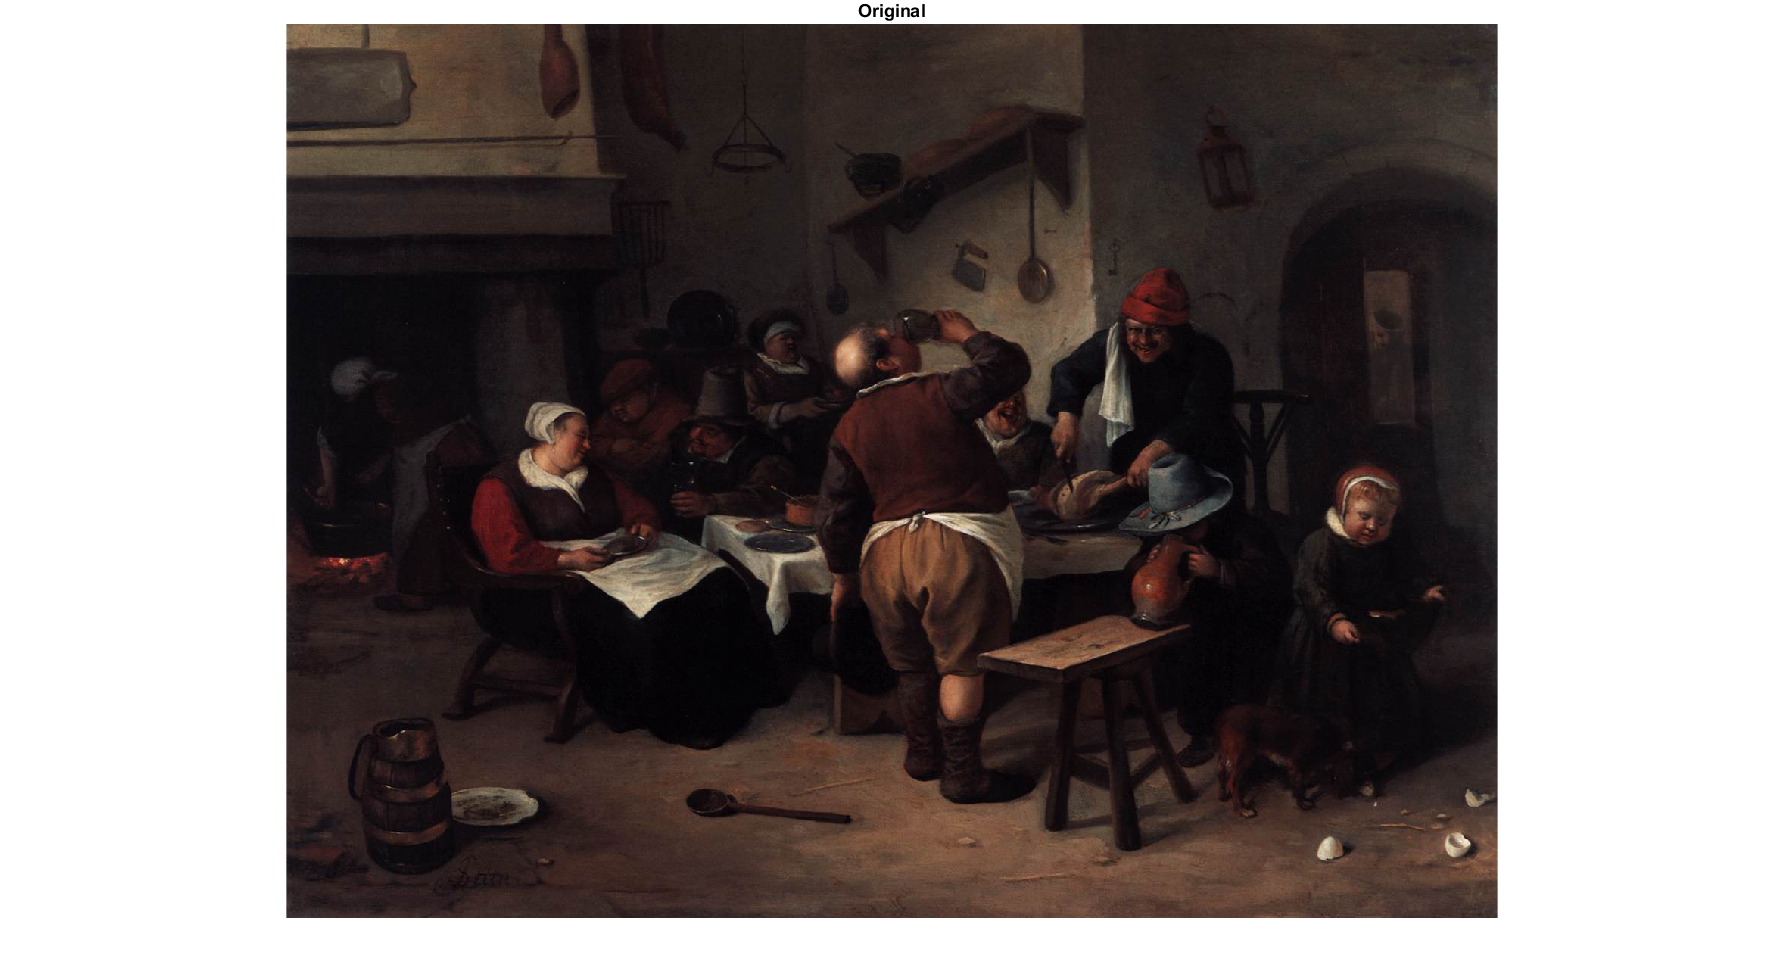
\includegraphics[width=1\linewidth]{inteq11.png}\par 
    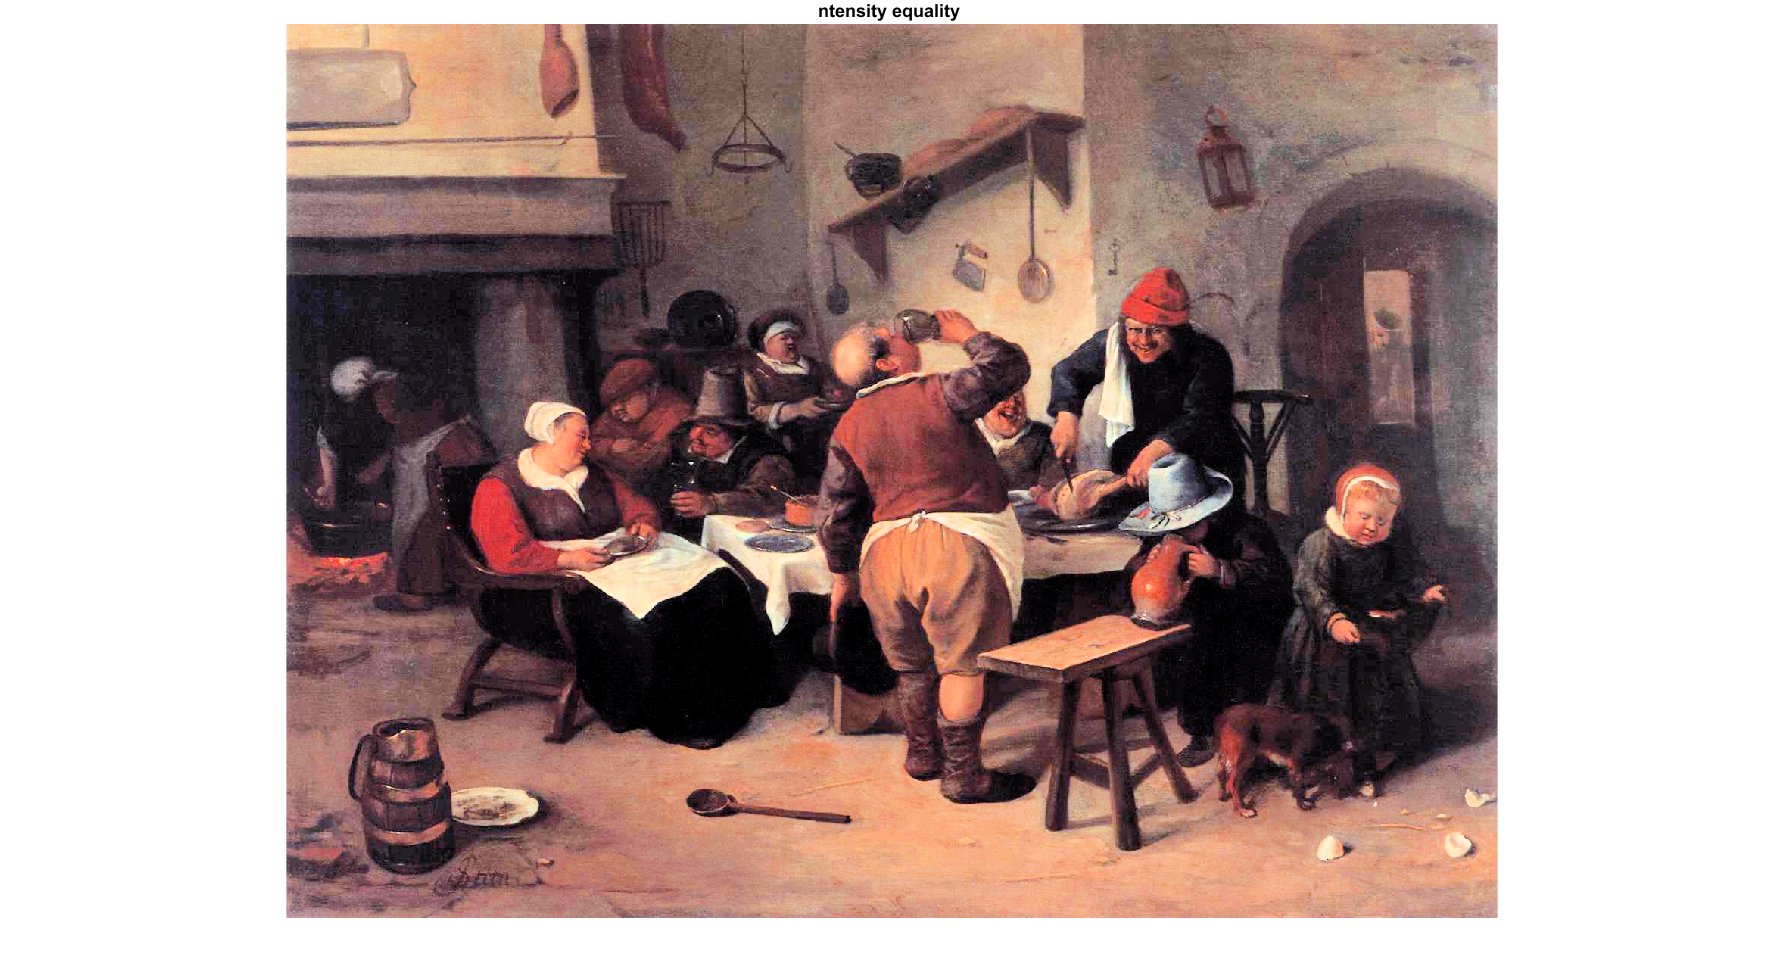
\includegraphics[width=1\linewidth]{inteq12.png}\par 
    \end{multicols}
\caption{Intensity equalization obtained by equalization only on luminance or value channel. Original image (left), results of intensity equalization (right)}
\label{int_1}
\end{figure*}

\begin{figure*}[ht]
\begin{multicols}{2}
    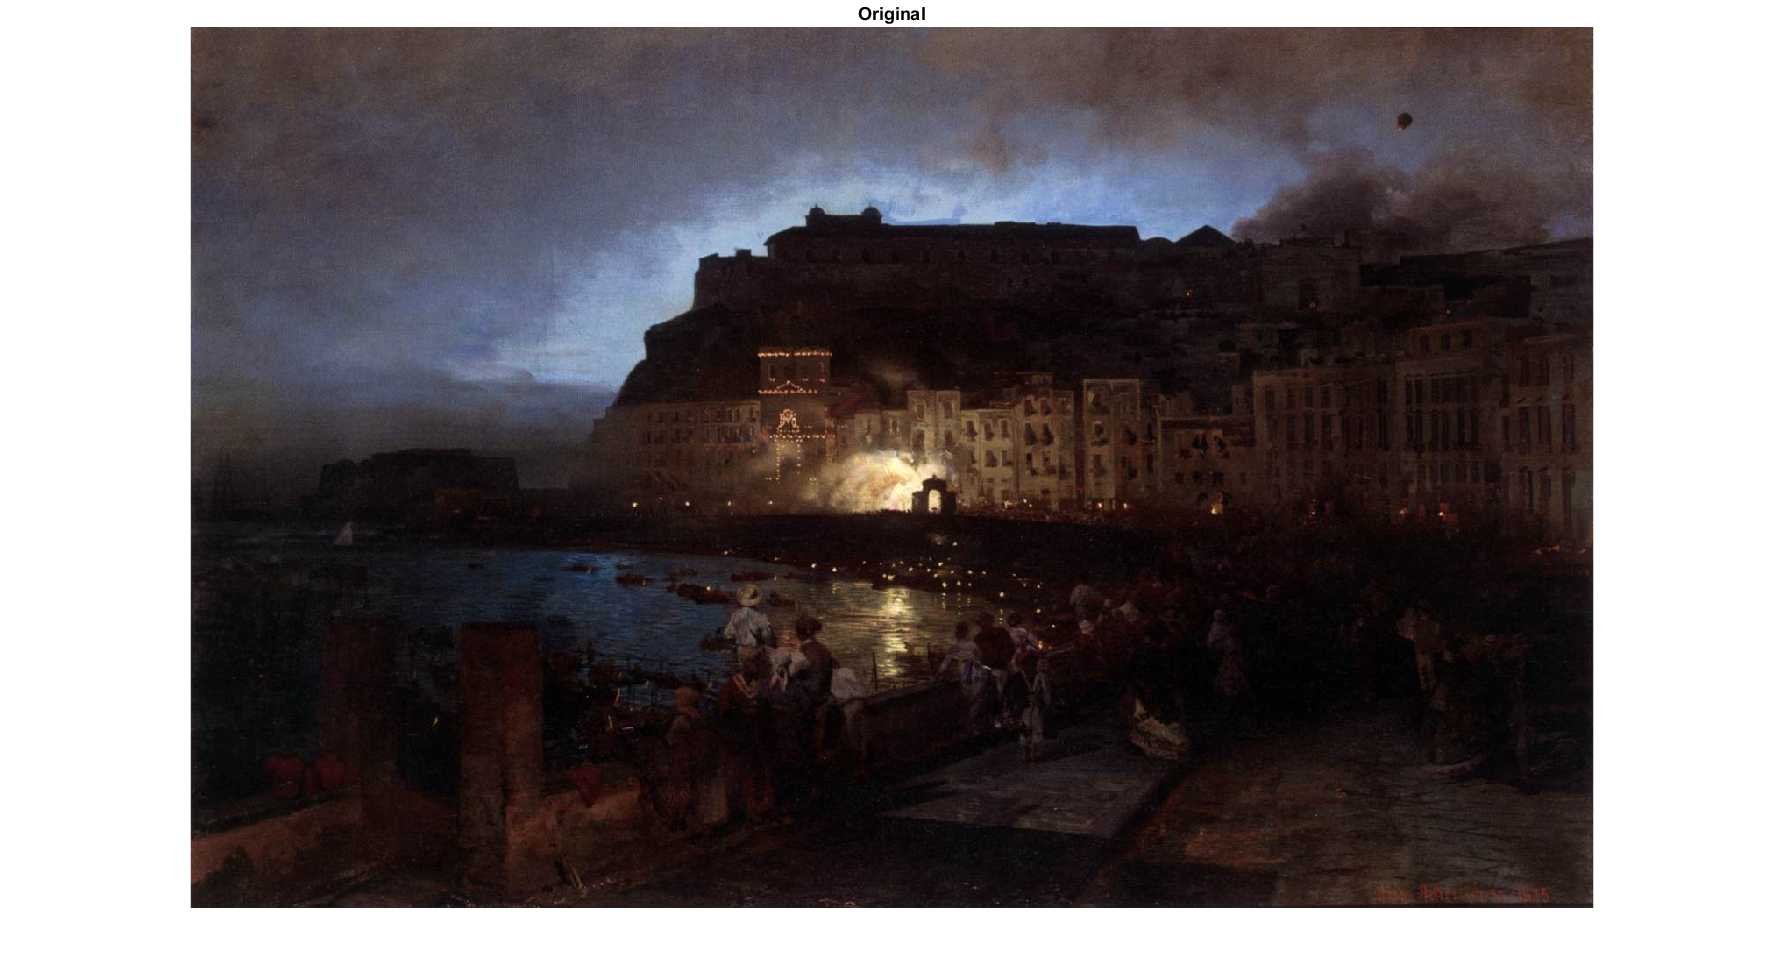
\includegraphics[width=\linewidth]{inteq21.png}\par 
    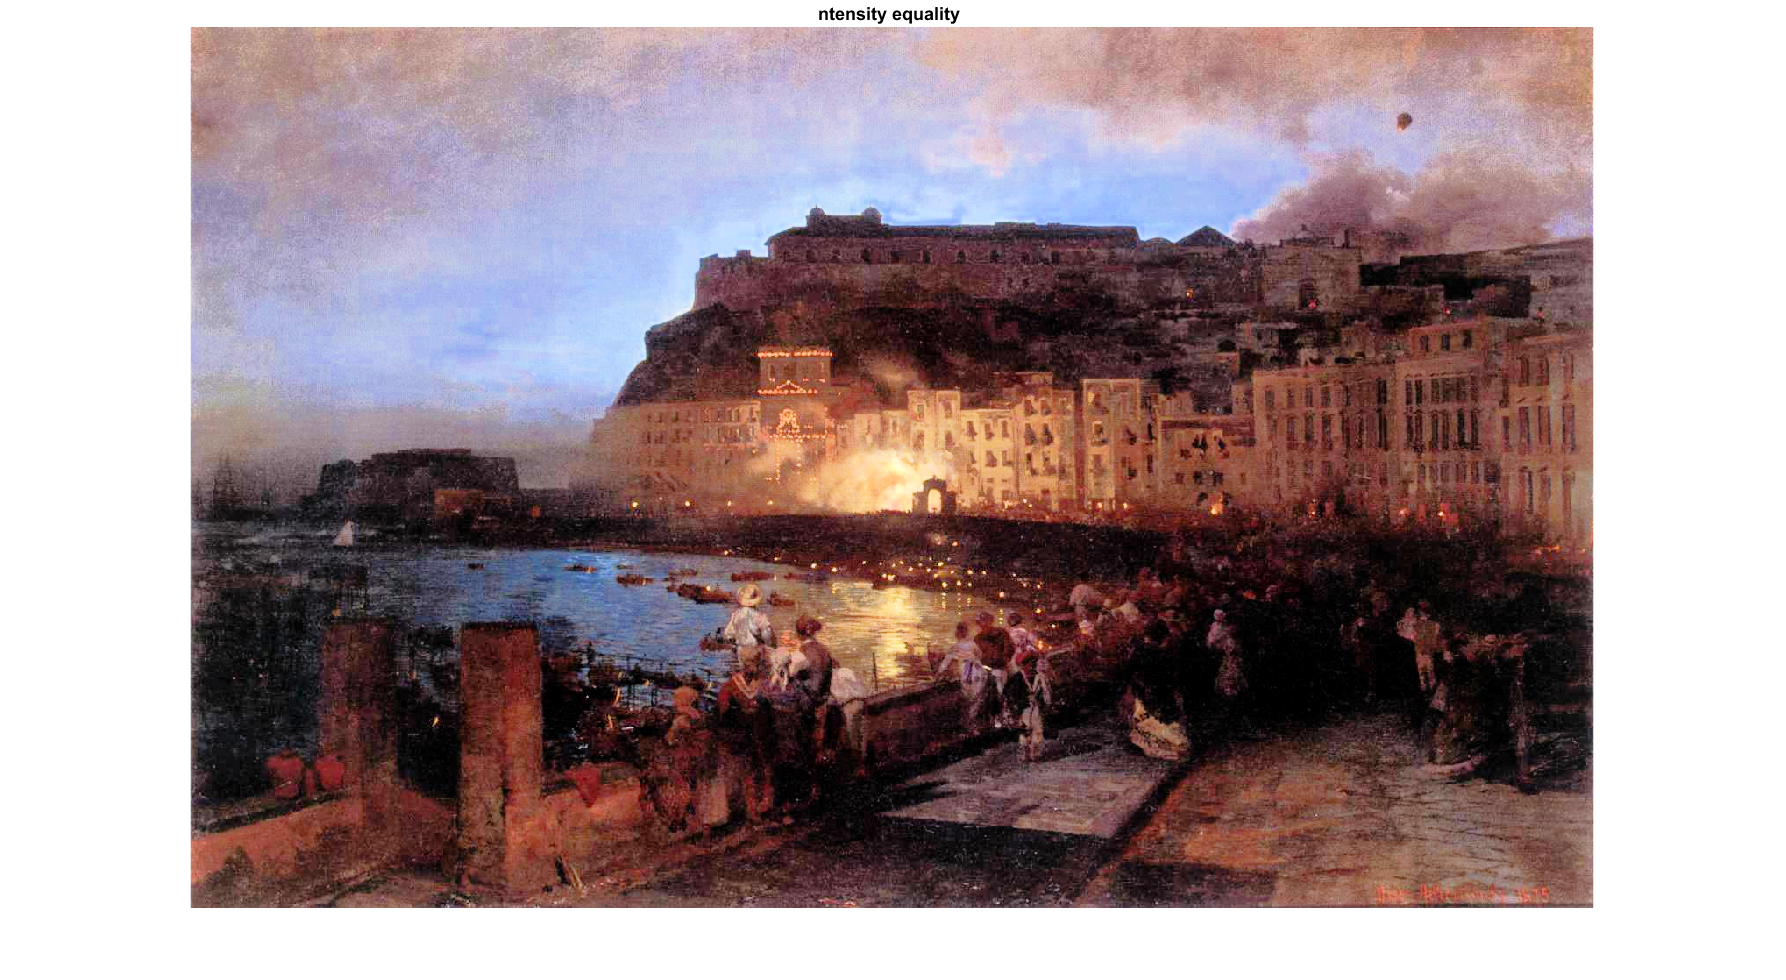
\includegraphics[width=\linewidth]{inteq22.png}\par 
    \end{multicols}
\caption{Intensity equalization obtained by equalization only on luminance or value channel. Original image (left), results of intensity equalization (right)}
\label{int_2}
\end{figure*}

\begin{figure*}[ht]
\begin{multicols}{2}
    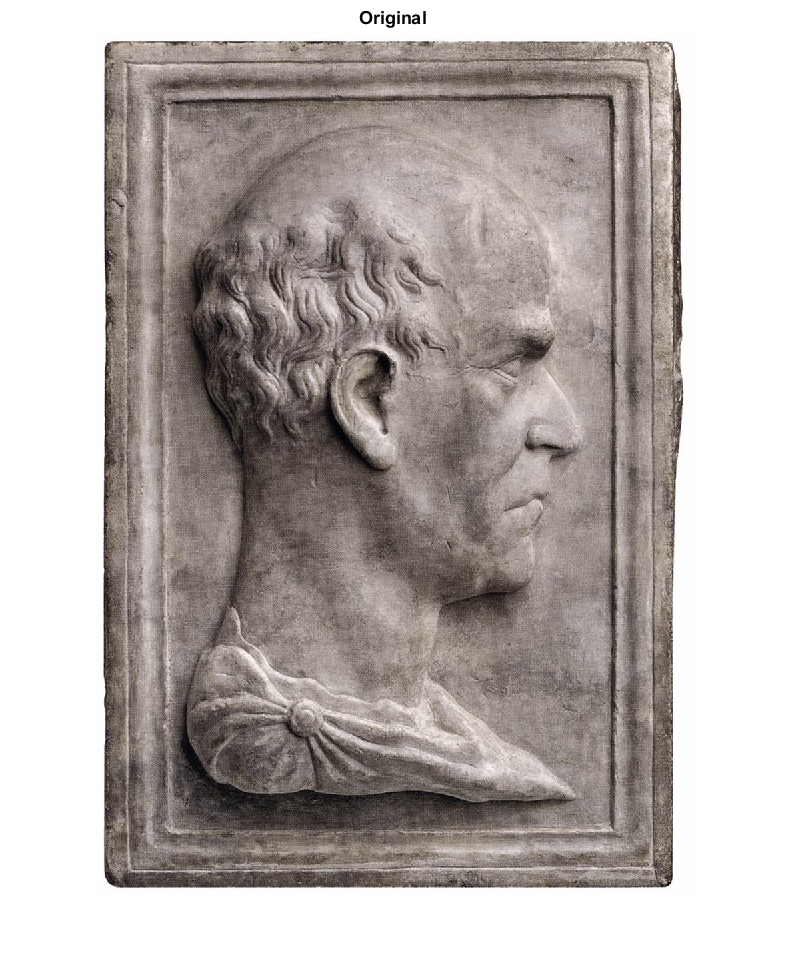
\includegraphics[width=\linewidth]{histeq11.png}\par 
    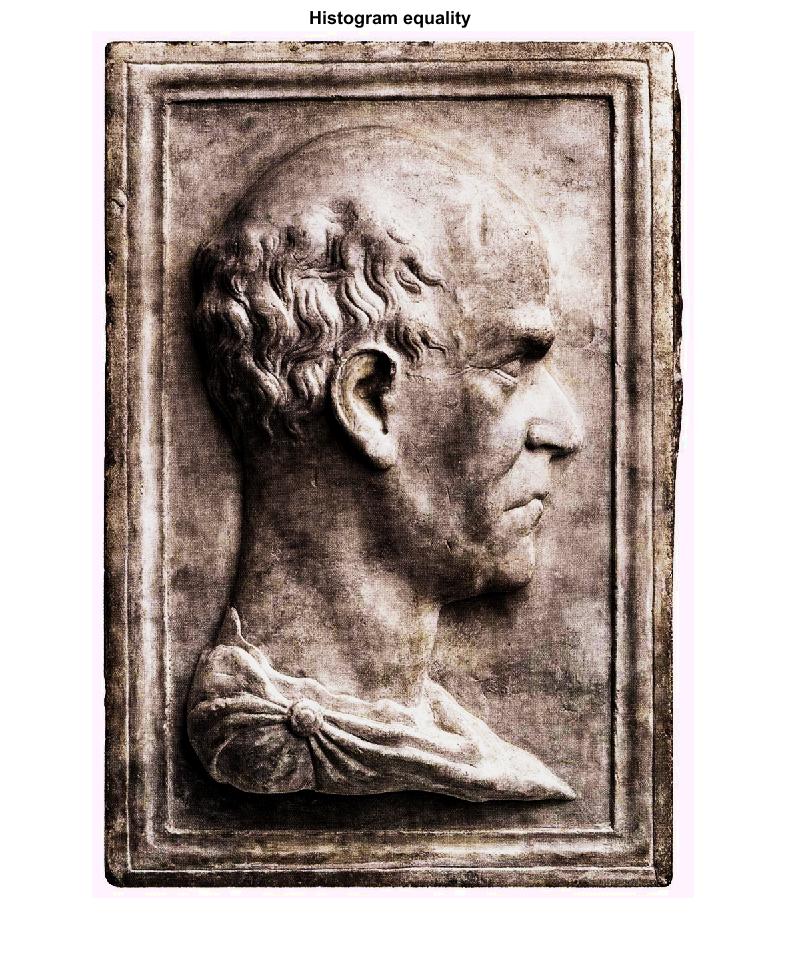
\includegraphics[width=\linewidth]{histeq12.png}\par 
    \end{multicols}
\caption{Histogram equalization on RGB channels. Original image (left), results of histogram equalization (right)}
\label{hist_1}
\end{figure*}

\begin{figure*}[ht]
\begin{multicols}{2}
    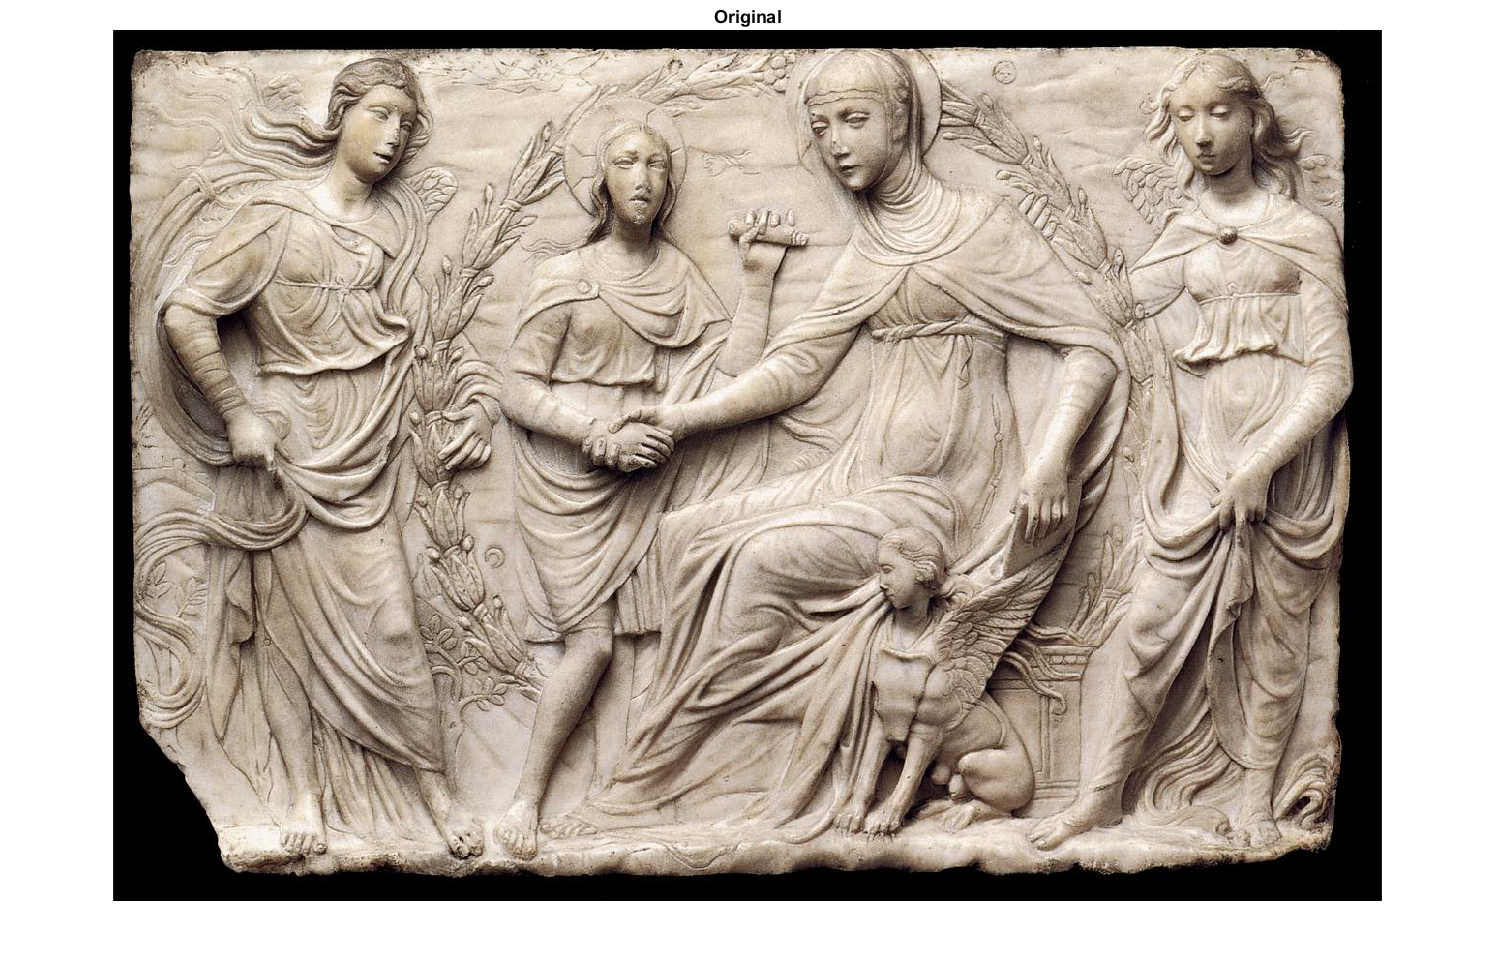
\includegraphics[width=\linewidth]{histeq21.png}\par 
    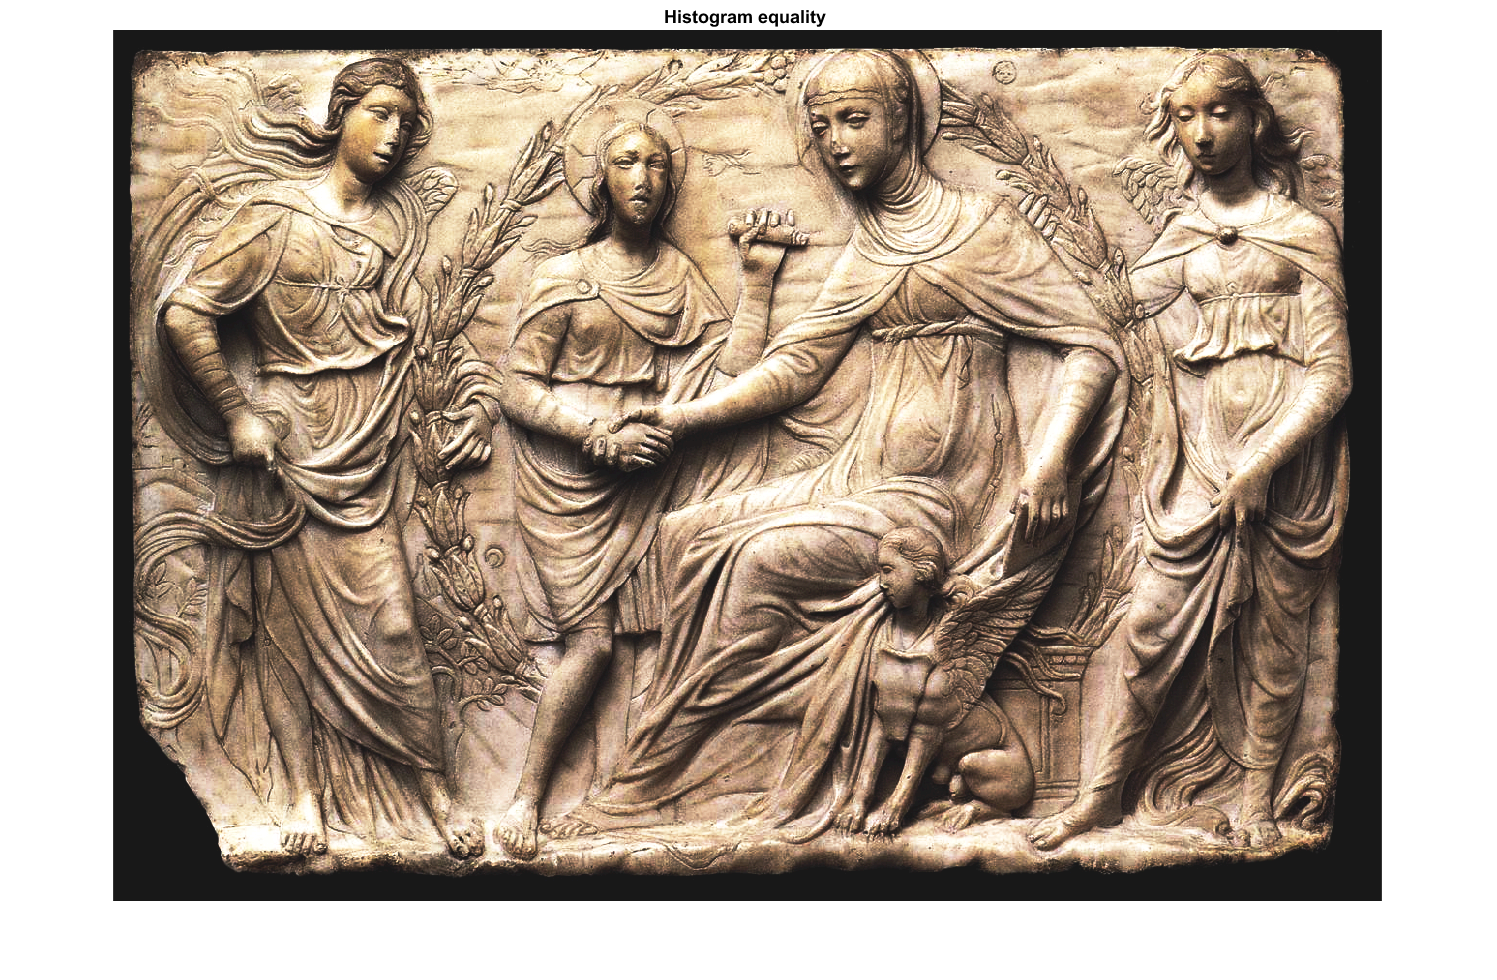
\includegraphics[width=\linewidth]{histeq22.png}\par 
    \end{multicols}
\caption{Histogram equalization on RGB channels. Original image (left), results of histogram equalization (right)}
\label{hist_2}
\end{figure*}



\begin{figure*}[ht]
\begin{multicols}{2}
    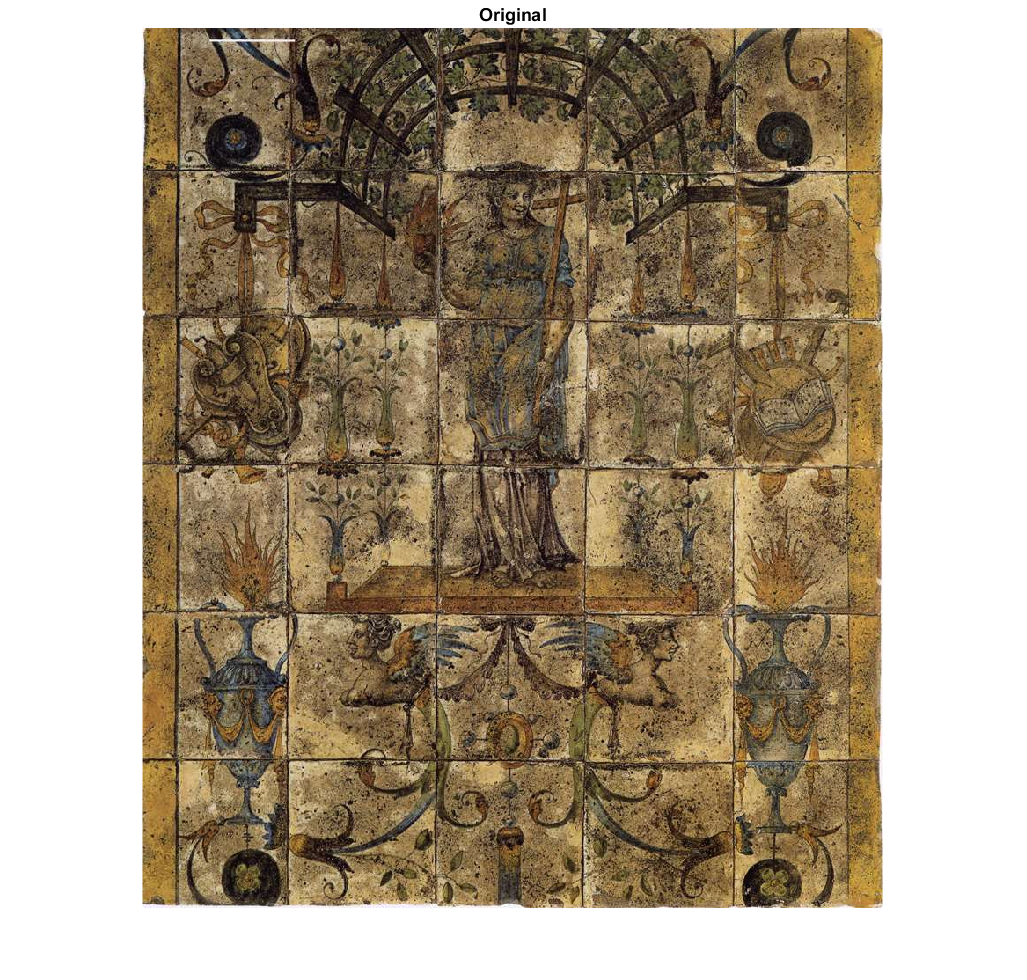
\includegraphics[width=\linewidth]{med11.png}\par 
    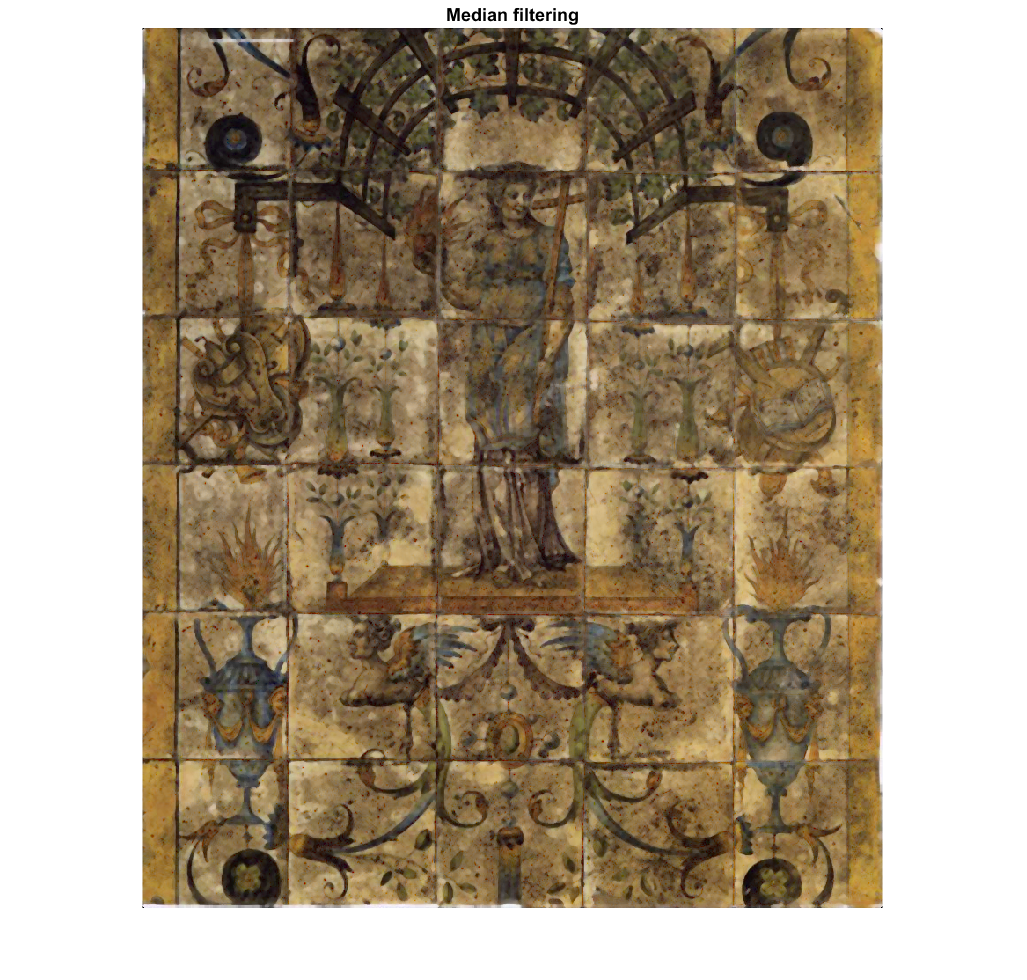
\includegraphics[width=\linewidth]{med12.png}\par 
    \end{multicols}
\caption{Filtering the spike noise using median filter. Original image (left), results of median filter (right)}
\label{med_1}
\end{figure*}


\begin{figure*}[ht]
\begin{multicols}{2}
    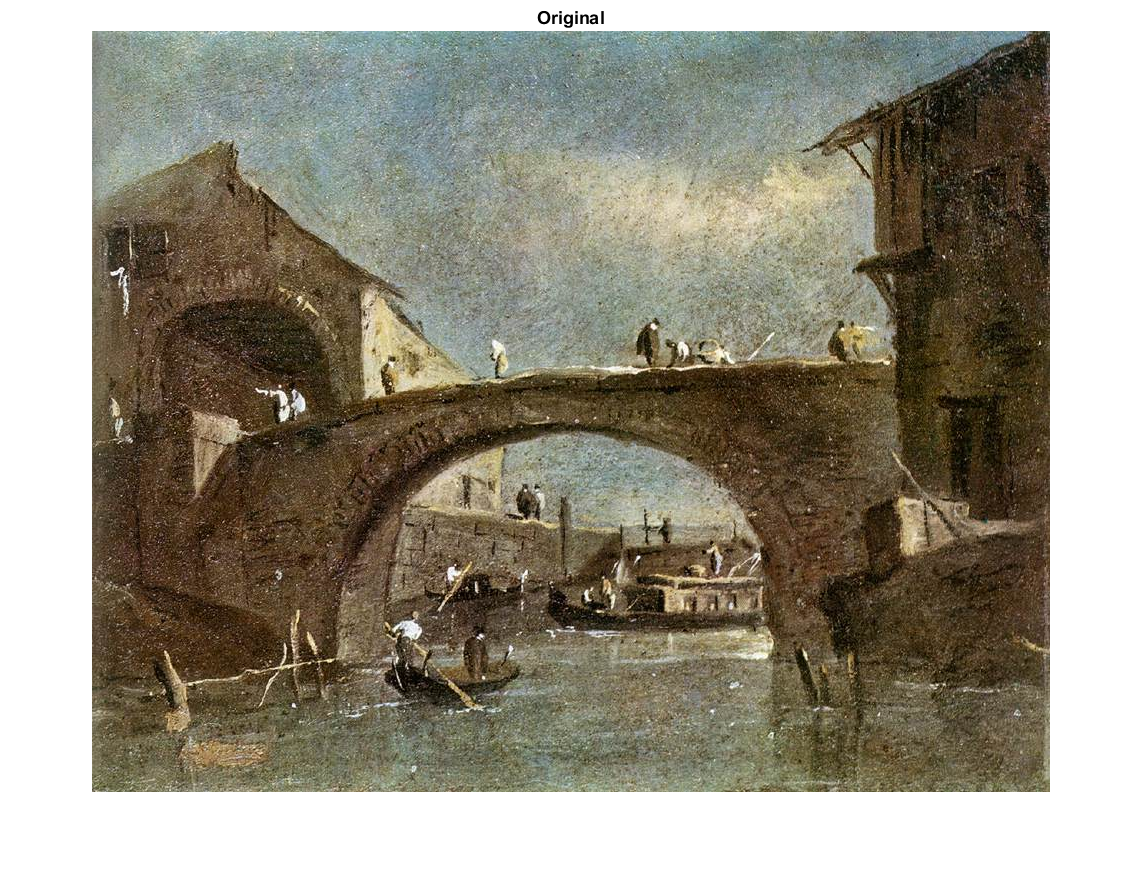
\includegraphics[width=\linewidth]{med21.png}\par 
    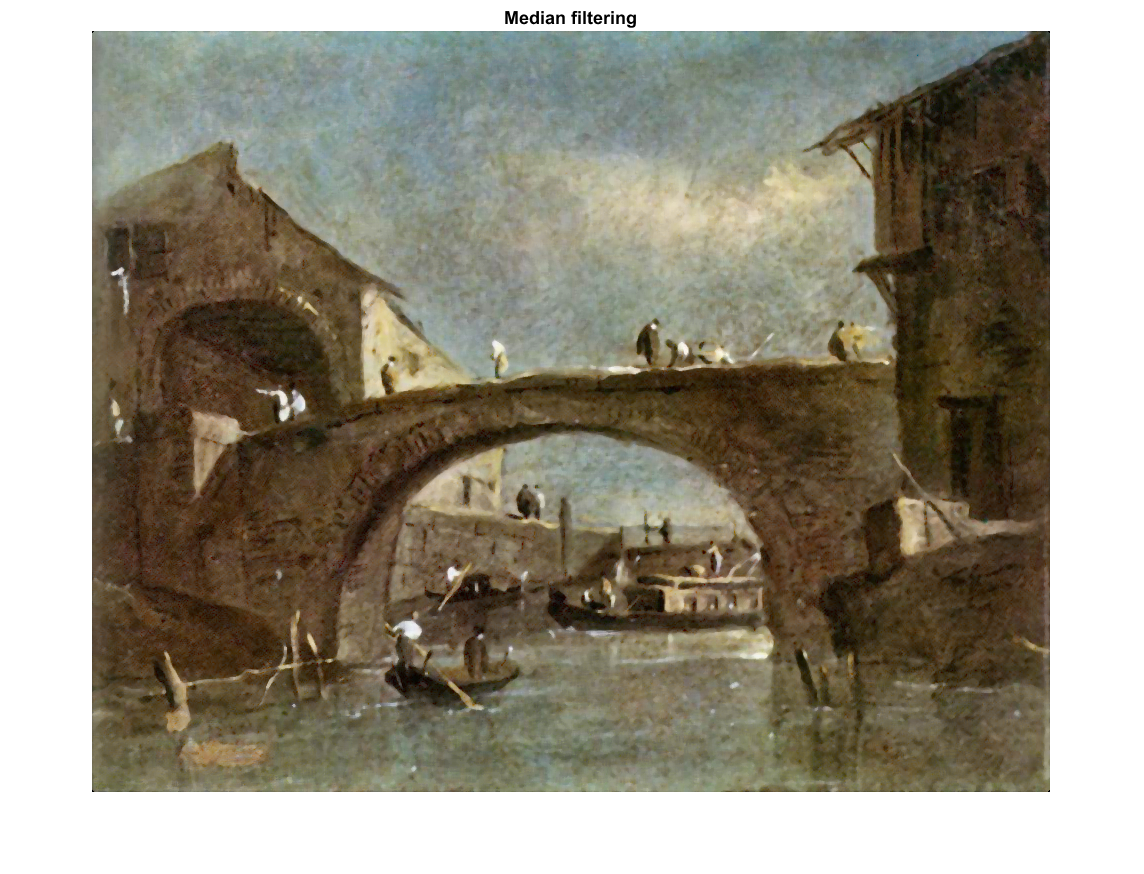
\includegraphics[width=\linewidth]{med22.png}\par 
    \end{multicols}
\caption{Filtering the spike noise using median filter. Original image (left), results of median filter (right)}
\label{med_2}
\end{figure*}


\begin{figure*}[ht]
\begin{multicols}{2}
    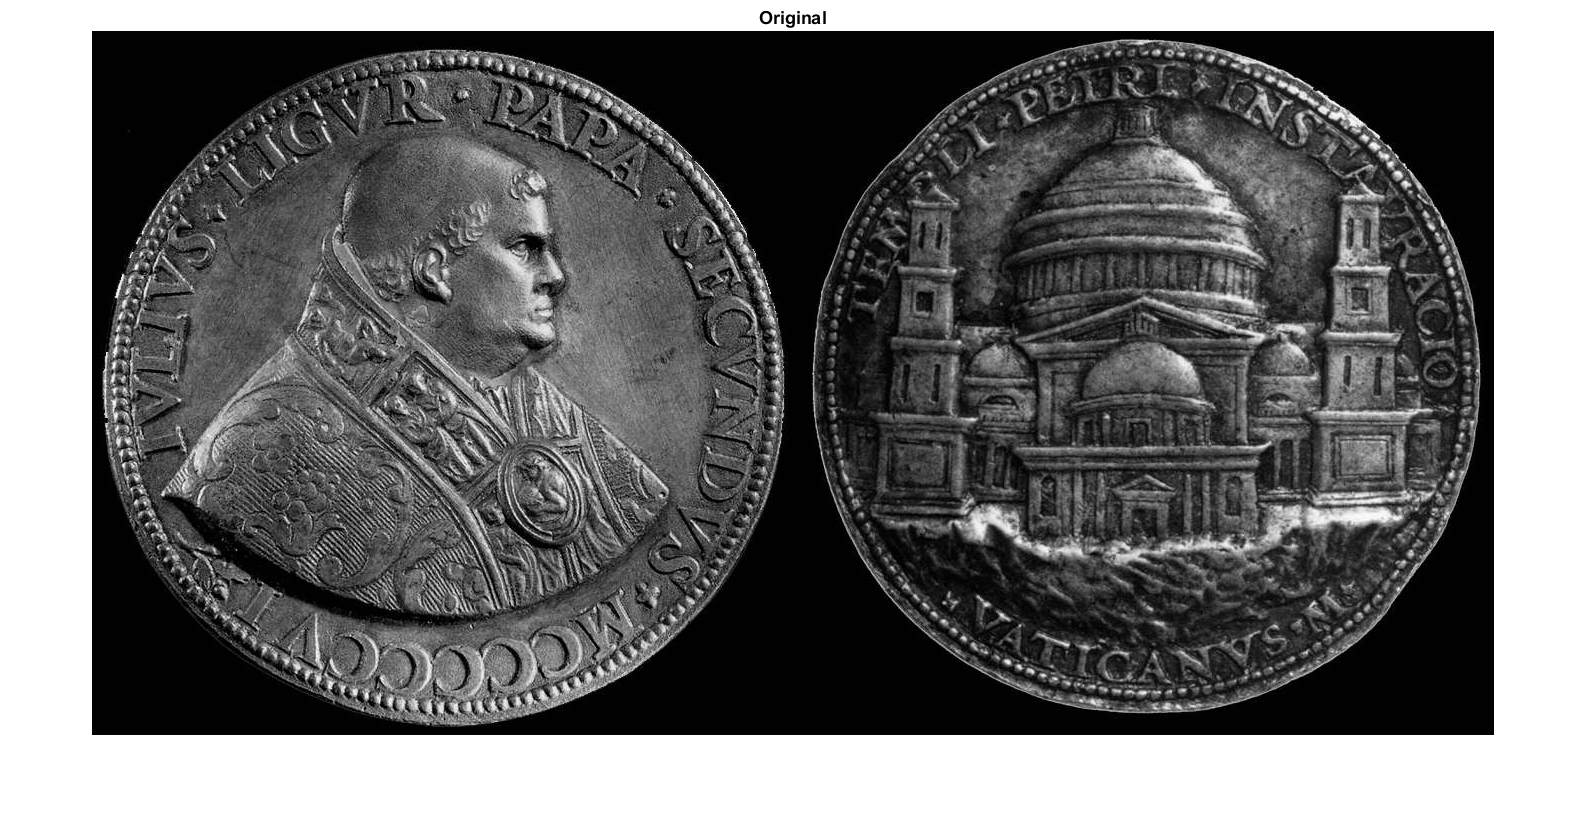
\includegraphics[width=1.1\linewidth]{colmap11.png}\par 
    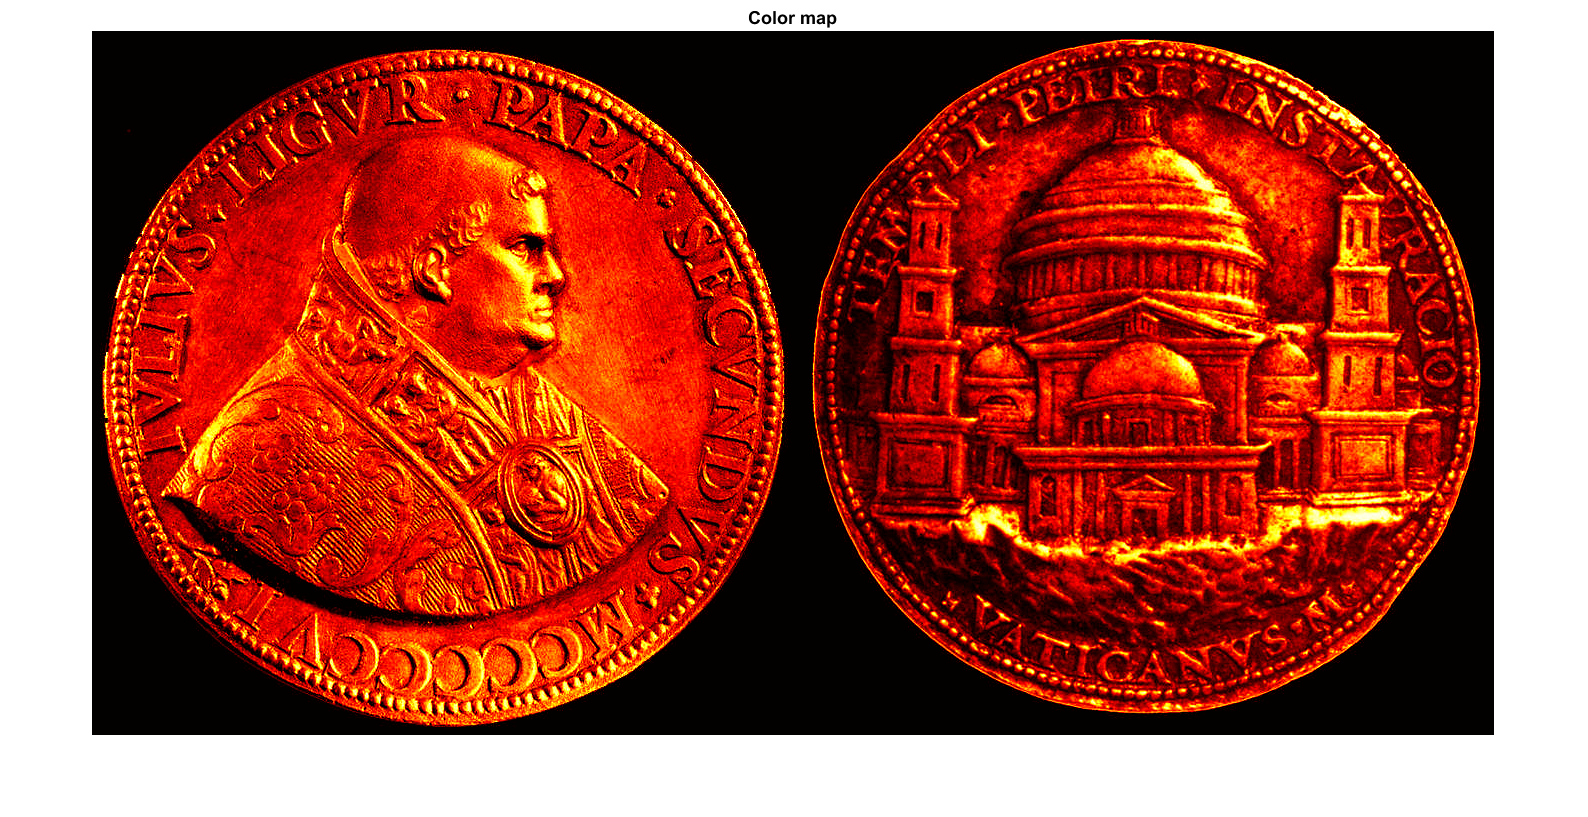
\includegraphics[width=1.1\linewidth]{colmap12.png}\par 
    \end{multicols}
\caption{Pseudo-color enhancement by using the gray-level to color transformation. Original image (left), results obtained with colormap `hot' (right)}
\label{colmap_1}
\end{figure*}


\begin{figure*}[ht]
\begin{multicols}{2}
    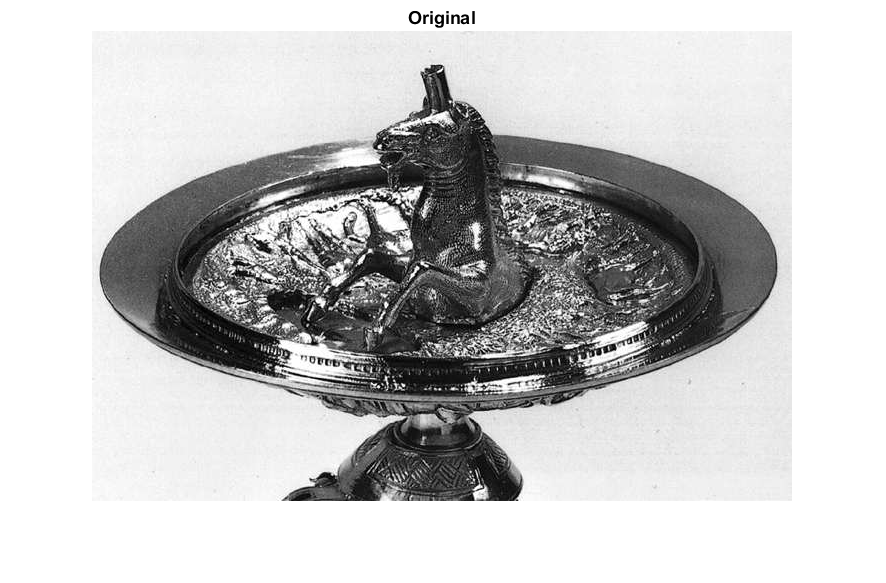
\includegraphics[width=1.1\linewidth]{colmap21.png}\par 
    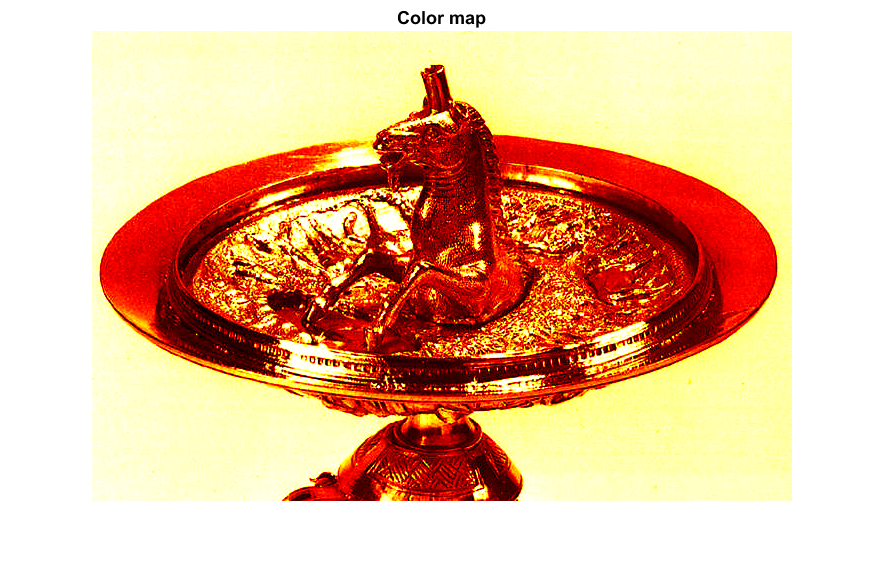
\includegraphics[width=1.1\linewidth]{colmap22.png}\par 
    \end{multicols}
\caption{Pseudo-color enhancement by using the gray-level to color transformation. Original image (left), results obtained with colormap `hot' (right)}
\label{colmap_2}
\end{figure*}

\begin{figure*}[ht]
\begin{multicols}{2}
    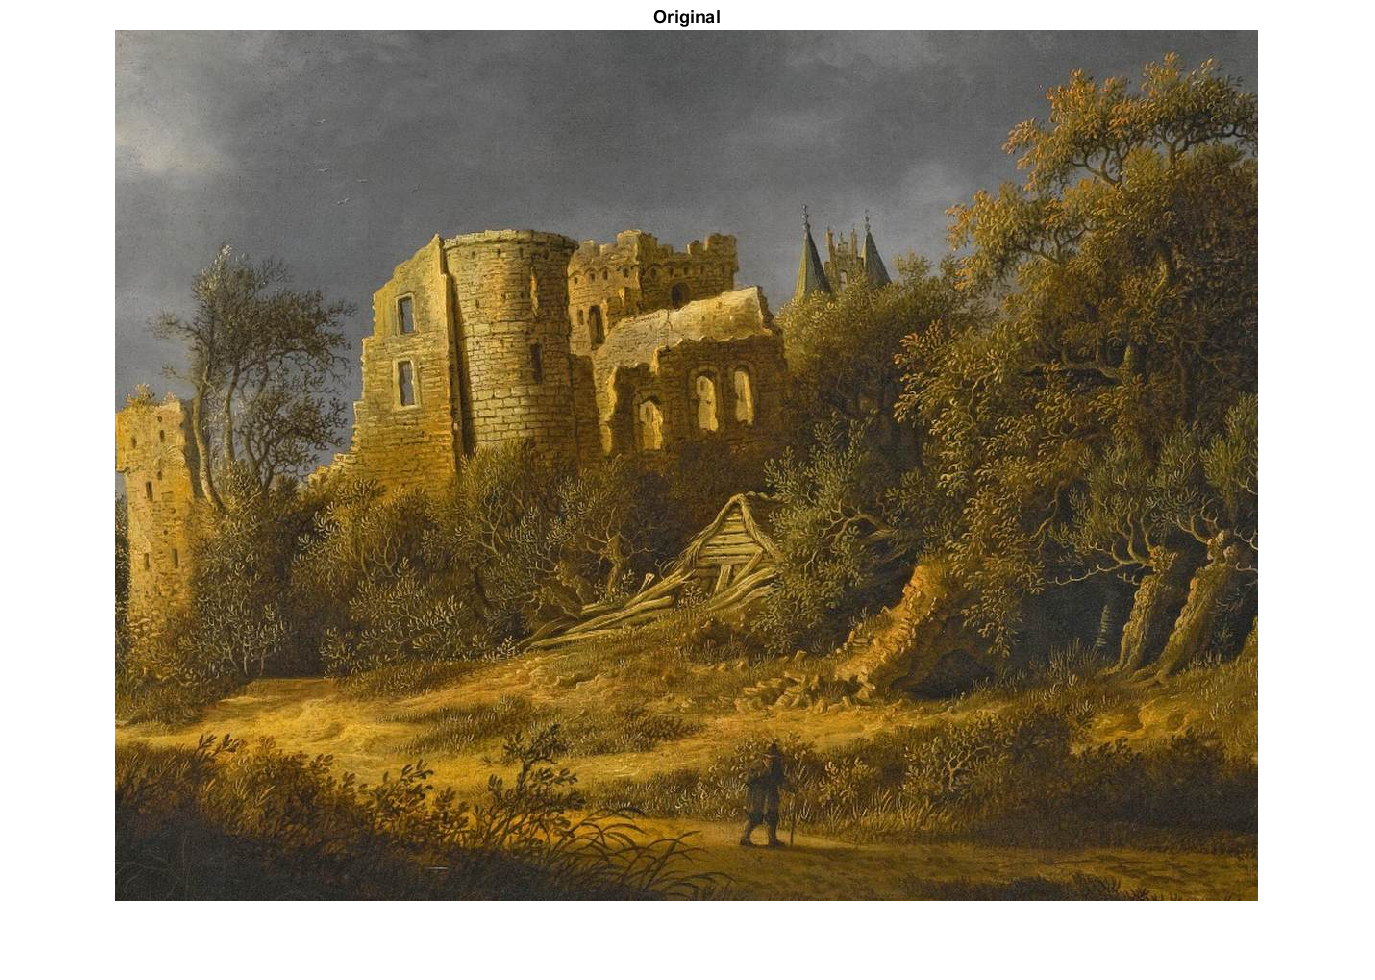
\includegraphics[width=\linewidth]{colbal11.png}\par 
    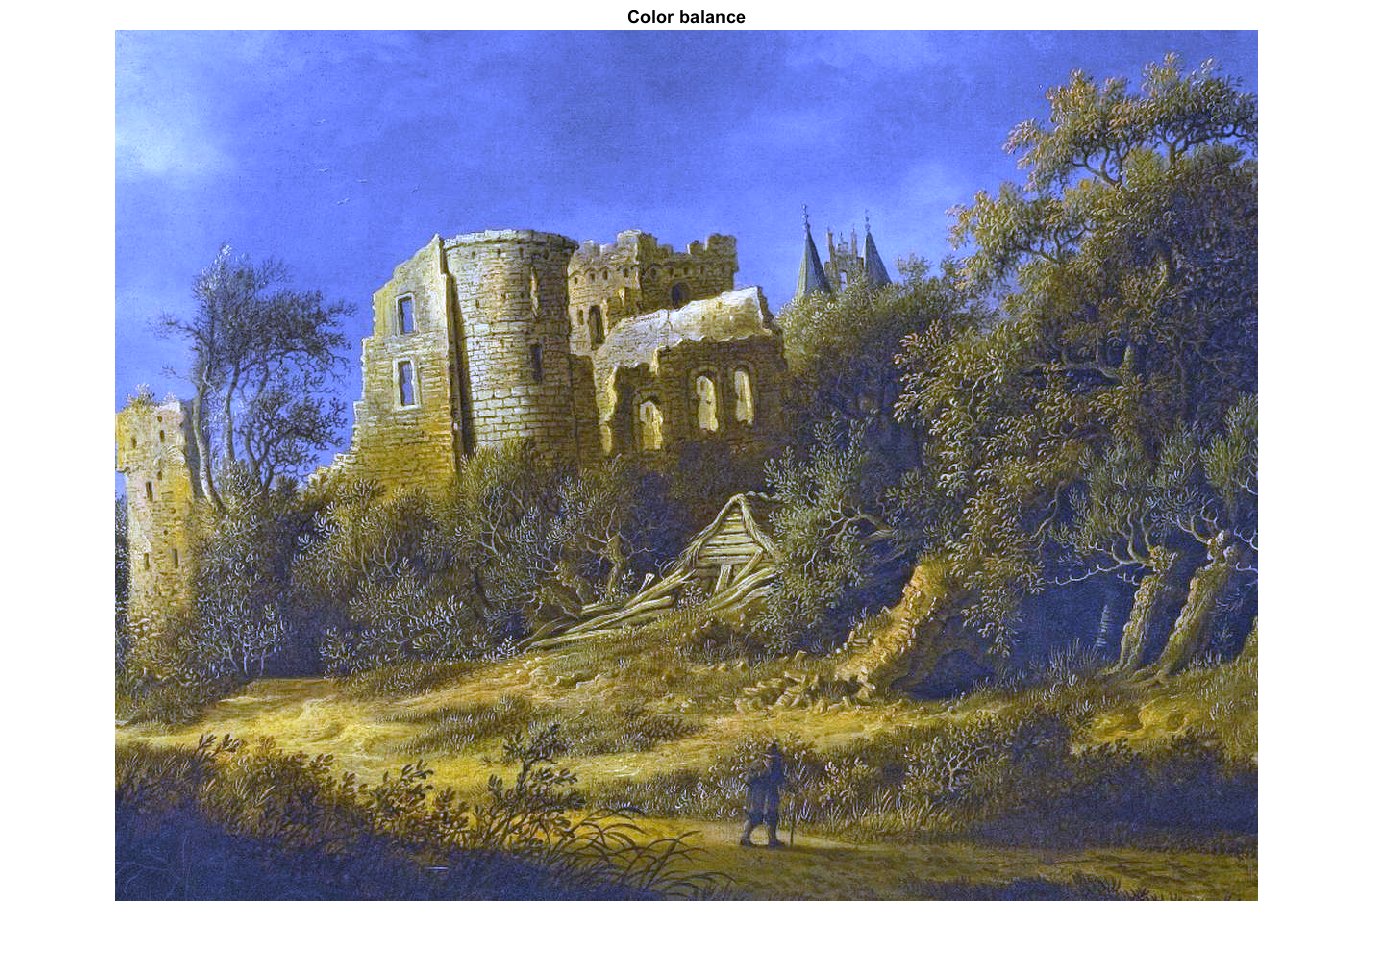
\includegraphics[width=\linewidth]{colbal12.png}\par 
    \end{multicols}
\caption{Color balance of image using the algorithm in \cite{colbal}. Original image (left), results of color balancing (right)}
\label{colbal_1}
\end{figure*}


\begin{figure*}[ht]
\begin{multicols}{2}
    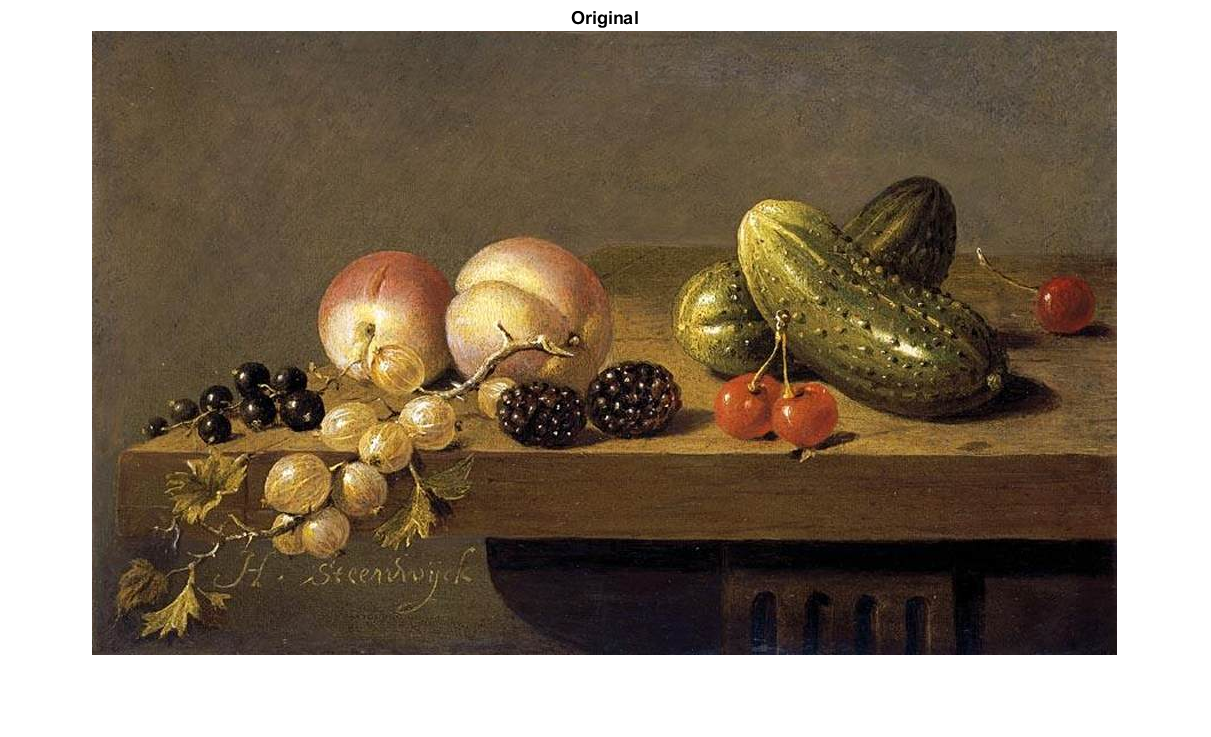
\includegraphics[width=\linewidth]{colbal21.png}\par 
    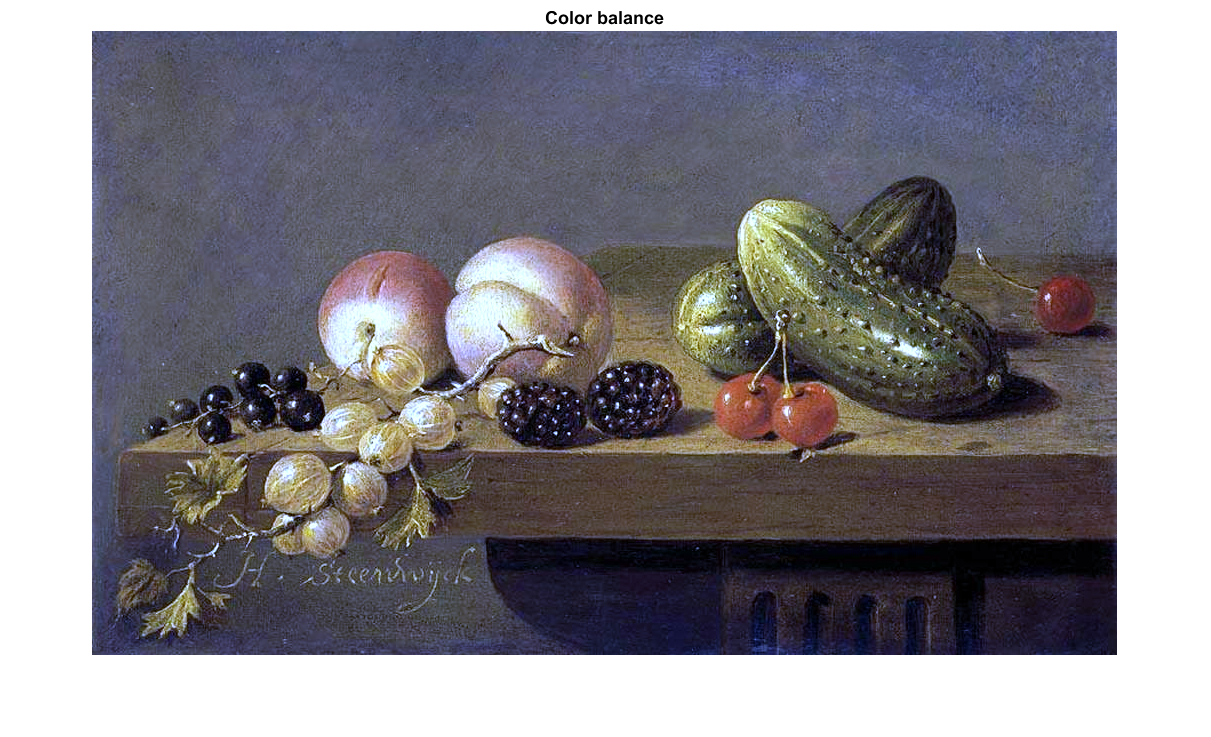
\includegraphics[width=\linewidth]{colbal22.png}\par 
    \end{multicols}
\caption{Color balance of image using the algorithm in \cite{colbal}. Original image (left), results of color balancing (right)}
\label{colbal_2}
\end{figure*}


%
%\begin{figure}[htbp]
%\centerline{\includegraphics{inteq1.png}}
%\caption{Example of a figure caption.}
%\label{fig}
%\end{figure}


%\begin{figure}[htbp]
%\centerline{\includegraphics{inteq2.png}}
%\caption{Example of a figure caption.}
%\label{fig}
%\end{figure}



\begin{thebibliography}{00}
\bibitem{poole} Poole, David, and Le-Phat Ho. "Digital transitions and the impact of new technology on the arts." Canadian Public Arts Funders Network (2011): 2-64.
\bibitem{gonzalez} Gonzalez, Rafael C., and Richard E. Woods. "Digital image processing prentice hall." Upper Saddle River, NJ (2002).
\bibitem{angel} https://angeljohnsy.blogspot.com/2016/03/gray-scale-to-pseudo-color.html
\bibitem{wikiColorBalance} https://en.wikipedia.org/wiki/Color-balance
\bibitem{colbal} https://se.mathworks.com/matlabcentral/fileexchange/14294-program-color-balancing



\end{thebibliography}

\end{document}
